% Options for packages loaded elsewhere
\PassOptionsToPackage{unicode}{hyperref}
\PassOptionsToPackage{hyphens}{url}
%
\documentclass[
]{article}
\usepackage{amsmath,amssymb}
\usepackage{lmodern}
\usepackage{iftex}
\ifPDFTeX
  \usepackage[T1]{fontenc}
  \usepackage[utf8]{inputenc}
  \usepackage{textcomp} % provide euro and other symbols
\else % if luatex or xetex
  \usepackage{unicode-math}
  \defaultfontfeatures{Scale=MatchLowercase}
  \defaultfontfeatures[\rmfamily]{Ligatures=TeX,Scale=1}
\fi
% Use upquote if available, for straight quotes in verbatim environments
\IfFileExists{upquote.sty}{\usepackage{upquote}}{}
\IfFileExists{microtype.sty}{% use microtype if available
  \usepackage[]{microtype}
  \UseMicrotypeSet[protrusion]{basicmath} % disable protrusion for tt fonts
}{}
\makeatletter
\@ifundefined{KOMAClassName}{% if non-KOMA class
  \IfFileExists{parskip.sty}{%
    \usepackage{parskip}
  }{% else
    \setlength{\parindent}{0pt}
    \setlength{\parskip}{6pt plus 2pt minus 1pt}}
}{% if KOMA class
  \KOMAoptions{parskip=half}}
\makeatother
\usepackage{xcolor}
\usepackage[margin=1in]{geometry}
\usepackage{color}
\usepackage{fancyvrb}
\newcommand{\VerbBar}{|}
\newcommand{\VERB}{\Verb[commandchars=\\\{\}]}
\DefineVerbatimEnvironment{Highlighting}{Verbatim}{commandchars=\\\{\}}
% Add ',fontsize=\small' for more characters per line
\usepackage{framed}
\definecolor{shadecolor}{RGB}{248,248,248}
\newenvironment{Shaded}{\begin{snugshade}}{\end{snugshade}}
\newcommand{\AlertTok}[1]{\textcolor[rgb]{0.94,0.16,0.16}{#1}}
\newcommand{\AnnotationTok}[1]{\textcolor[rgb]{0.56,0.35,0.01}{\textbf{\textit{#1}}}}
\newcommand{\AttributeTok}[1]{\textcolor[rgb]{0.77,0.63,0.00}{#1}}
\newcommand{\BaseNTok}[1]{\textcolor[rgb]{0.00,0.00,0.81}{#1}}
\newcommand{\BuiltInTok}[1]{#1}
\newcommand{\CharTok}[1]{\textcolor[rgb]{0.31,0.60,0.02}{#1}}
\newcommand{\CommentTok}[1]{\textcolor[rgb]{0.56,0.35,0.01}{\textit{#1}}}
\newcommand{\CommentVarTok}[1]{\textcolor[rgb]{0.56,0.35,0.01}{\textbf{\textit{#1}}}}
\newcommand{\ConstantTok}[1]{\textcolor[rgb]{0.00,0.00,0.00}{#1}}
\newcommand{\ControlFlowTok}[1]{\textcolor[rgb]{0.13,0.29,0.53}{\textbf{#1}}}
\newcommand{\DataTypeTok}[1]{\textcolor[rgb]{0.13,0.29,0.53}{#1}}
\newcommand{\DecValTok}[1]{\textcolor[rgb]{0.00,0.00,0.81}{#1}}
\newcommand{\DocumentationTok}[1]{\textcolor[rgb]{0.56,0.35,0.01}{\textbf{\textit{#1}}}}
\newcommand{\ErrorTok}[1]{\textcolor[rgb]{0.64,0.00,0.00}{\textbf{#1}}}
\newcommand{\ExtensionTok}[1]{#1}
\newcommand{\FloatTok}[1]{\textcolor[rgb]{0.00,0.00,0.81}{#1}}
\newcommand{\FunctionTok}[1]{\textcolor[rgb]{0.00,0.00,0.00}{#1}}
\newcommand{\ImportTok}[1]{#1}
\newcommand{\InformationTok}[1]{\textcolor[rgb]{0.56,0.35,0.01}{\textbf{\textit{#1}}}}
\newcommand{\KeywordTok}[1]{\textcolor[rgb]{0.13,0.29,0.53}{\textbf{#1}}}
\newcommand{\NormalTok}[1]{#1}
\newcommand{\OperatorTok}[1]{\textcolor[rgb]{0.81,0.36,0.00}{\textbf{#1}}}
\newcommand{\OtherTok}[1]{\textcolor[rgb]{0.56,0.35,0.01}{#1}}
\newcommand{\PreprocessorTok}[1]{\textcolor[rgb]{0.56,0.35,0.01}{\textit{#1}}}
\newcommand{\RegionMarkerTok}[1]{#1}
\newcommand{\SpecialCharTok}[1]{\textcolor[rgb]{0.00,0.00,0.00}{#1}}
\newcommand{\SpecialStringTok}[1]{\textcolor[rgb]{0.31,0.60,0.02}{#1}}
\newcommand{\StringTok}[1]{\textcolor[rgb]{0.31,0.60,0.02}{#1}}
\newcommand{\VariableTok}[1]{\textcolor[rgb]{0.00,0.00,0.00}{#1}}
\newcommand{\VerbatimStringTok}[1]{\textcolor[rgb]{0.31,0.60,0.02}{#1}}
\newcommand{\WarningTok}[1]{\textcolor[rgb]{0.56,0.35,0.01}{\textbf{\textit{#1}}}}
\usepackage{graphicx}
\makeatletter
\def\maxwidth{\ifdim\Gin@nat@width>\linewidth\linewidth\else\Gin@nat@width\fi}
\def\maxheight{\ifdim\Gin@nat@height>\textheight\textheight\else\Gin@nat@height\fi}
\makeatother
% Scale images if necessary, so that they will not overflow the page
% margins by default, and it is still possible to overwrite the defaults
% using explicit options in \includegraphics[width, height, ...]{}
\setkeys{Gin}{width=\maxwidth,height=\maxheight,keepaspectratio}
% Set default figure placement to htbp
\makeatletter
\def\fps@figure{htbp}
\makeatother
\setlength{\emergencystretch}{3em} % prevent overfull lines
\providecommand{\tightlist}{%
  \setlength{\itemsep}{0pt}\setlength{\parskip}{0pt}}
\setcounter{secnumdepth}{-\maxdimen} % remove section numbering
\ifLuaTeX
  \usepackage{selnolig}  % disable illegal ligatures
\fi
\IfFileExists{bookmark.sty}{\usepackage{bookmark}}{\usepackage{hyperref}}
\IfFileExists{xurl.sty}{\usepackage{xurl}}{} % add URL line breaks if available
\urlstyle{same} % disable monospaced font for URLs
\hypersetup{
  pdftitle={VADeaths},
  pdfauthor={coop711},
  hidelinks,
  pdfcreator={LaTeX via pandoc}}

\title{VADeaths}
\author{coop711}
\date{}

\begin{document}
\maketitle

\hypertarget{tidy-data}{%
\subsection{Tidy Data}\label{tidy-data}}

깔끔한(tidy) 데이터를 만드는 방법에 대하여 알아본다. 사용되는 데이터는
\texttt{R}에 내장되어 있는 \texttt{VADeaths} 이다. 이 데이터의 구조는
5세 간격의 연령대를 행의 이름으로 하고, 장소(Rural, Urban)와 성별(Male,
Female)의 조합을 열의 이름으로 갖는 행렬임을 알 수 있다.

\begin{Shaded}
\begin{Highlighting}[]
\NormalTok{VADeaths}
\end{Highlighting}
\end{Shaded}

\begin{verbatim}
##       Rural Male Rural Female Urban Male Urban Female
## 50-54       11.7          8.7       15.4          8.4
## 55-59       18.1         11.7       24.3         13.6
## 60-64       26.9         20.3       37.0         19.3
## 65-69       41.0         30.9       54.6         35.1
## 70-74       66.0         54.3       71.1         50.0
\end{verbatim}

\begin{Shaded}
\begin{Highlighting}[]
\FunctionTok{str}\NormalTok{(VADeaths)}
\end{Highlighting}
\end{Shaded}

\begin{verbatim}
##  num [1:5, 1:4] 11.7 18.1 26.9 41 66 8.7 11.7 20.3 30.9 54.3 ...
##  - attr(*, "dimnames")=List of 2
##   ..$ : chr [1:5] "50-54" "55-59" "60-64" "65-69" ...
##   ..$ : chr [1:4] "Rural Male" "Rural Female" "Urban Male" "Urban Female"
\end{verbatim}

\hypertarget{base-r-uxc758-uxb3c4uxad6c-uxd65cuxc6a9}{%
\subsection{\texorpdfstring{\texttt{Base\ R} 의 도구
활용}{Base R 의 도구 활용}}\label{base-r-uxc758-uxb3c4uxad6c-uxd65cuxc6a9}}

왜 이 데이터가 깔끔하지(tidy) 않은지 생각해 보자. 데이터를 어떻게
표현해야 깔끔한 것인지 최종 결과물과 비교한다.

\texttt{c()}는 행렬 구조로 표현한 \texttt{VADeaths}를 기다란 하나의
벡터로 나타낸다. 이렇게 만든 한 줄의 벡터를 \texttt{Rates}에 옮겨
넣는다.

보통 \texttt{ordered()}가 아닌 \texttt{factor()}를 사용하는 경우가
많은데 연령이라는 변수의 특성을 감안하면 단순히 명목형이 아니고 엄연히
순서가 있기 때문에\texttt{ordered()}를 사용하는 것이 적절하다.

\begin{Shaded}
\begin{Highlighting}[]
\NormalTok{Rates }\OtherTok{\textless{}{-}} \FunctionTok{c}\NormalTok{(VADeaths)  }\DocumentationTok{\#\# 행렬를 한 줄의 벡터로 변환 }
\NormalTok{N }\OtherTok{\textless{}{-}} \FunctionTok{length}\NormalTok{(Rates) }\DocumentationTok{\#\# \textasciigrave{}Rates\textasciigrave{}의 크기를 \textasciigrave{}N\textasciigrave{}으로 저장.}
\NormalTok{Age }\OtherTok{\textless{}{-}} \FunctionTok{ordered}\NormalTok{(}\FunctionTok{rownames}\NormalTok{(VADeaths)) }\CommentTok{\# 행 이름으로 주어진 글자 벡터, 연령대를 순서형 범주로 변환. }
\NormalTok{Age }\OtherTok{\textless{}{-}} \FunctionTok{rep}\NormalTok{(}\FunctionTok{ordered}\NormalTok{(}\FunctionTok{rownames}\NormalTok{(VADeaths)), }\CommentTok{\# 전체 관찰 수효 만큼 반복. \textasciigrave{}length.out = \textasciigrave{}의 용례에 유의. }
           \AttributeTok{length.out =}\NormalTok{ N)}
\NormalTok{Place }\OtherTok{\textless{}{-}} \FunctionTok{gl}\NormalTok{(}\DecValTok{2}\NormalTok{, }\DecValTok{10}\NormalTok{, N, }\CommentTok{\# 농촌, 도시의 두 수준을 10번씩 반복하는 \textasciigrave{}factor\textasciigrave{} 설정}
           \AttributeTok{labels =} \FunctionTok{c}\NormalTok{(}\StringTok{"Rural"}\NormalTok{, }\StringTok{"Urban"}\NormalTok{))}
\NormalTok{Gender }\OtherTok{\textless{}{-}} \FunctionTok{gl}\NormalTok{(}\DecValTok{2}\NormalTok{, }\DecValTok{5}\NormalTok{, N, }\CommentTok{\# 성별은 5번씩 반복 }
             \AttributeTok{labels =} \FunctionTok{c}\NormalTok{(}\StringTok{"Male"}\NormalTok{, }\StringTok{"Female"}\NormalTok{))}
\FunctionTok{data.frame}\NormalTok{(Age, Place, Gender, Rates) }\CommentTok{\# 각 벡터를 데이터 프레임의 요소로 편성}
\end{Highlighting}
\end{Shaded}

\begin{verbatim}
##      Age Place Gender Rates
## 1  50-54 Rural   Male  11.7
## 2  55-59 Rural   Male  18.1
## 3  60-64 Rural   Male  26.9
## 4  65-69 Rural   Male  41.0
## 5  70-74 Rural   Male  66.0
## 6  50-54 Rural Female   8.7
## 7  55-59 Rural Female  11.7
## 8  60-64 Rural Female  20.3
## 9  65-69 Rural Female  30.9
## 10 70-74 Rural Female  54.3
## 11 50-54 Urban   Male  15.4
## 12 55-59 Urban   Male  24.3
## 13 60-64 Urban   Male  37.0
## 14 65-69 Urban   Male  54.6
## 15 70-74 Urban   Male  71.1
## 16 50-54 Urban Female   8.4
## 17 55-59 Urban Female  13.6
## 18 60-64 Urban Female  19.3
## 19 65-69 Urban Female  35.1
## 20 70-74 Urban Female  50.0
\end{verbatim}

\begin{Shaded}
\begin{Highlighting}[]
\NormalTok{VADeaths\_df }\OtherTok{\textless{}{-}} \FunctionTok{data.frame}\NormalTok{(Age, Place, Gender, Rates) }\CommentTok{\# 데이터 프레임을 새로운 R 객체로 지정 }
\NormalTok{VADeaths\_df }\CommentTok{\# 데이터 프레임 출력 }
\end{Highlighting}
\end{Shaded}

\begin{verbatim}
##      Age Place Gender Rates
## 1  50-54 Rural   Male  11.7
## 2  55-59 Rural   Male  18.1
## 3  60-64 Rural   Male  26.9
## 4  65-69 Rural   Male  41.0
## 5  70-74 Rural   Male  66.0
## 6  50-54 Rural Female   8.7
## 7  55-59 Rural Female  11.7
## 8  60-64 Rural Female  20.3
## 9  65-69 Rural Female  30.9
## 10 70-74 Rural Female  54.3
## 11 50-54 Urban   Male  15.4
## 12 55-59 Urban   Male  24.3
## 13 60-64 Urban   Male  37.0
## 14 65-69 Urban   Male  54.6
## 15 70-74 Urban   Male  71.1
## 16 50-54 Urban Female   8.4
## 17 55-59 Urban Female  13.6
## 18 60-64 Urban Female  19.3
## 19 65-69 Urban Female  35.1
## 20 70-74 Urban Female  50.0
\end{verbatim}

\begin{Shaded}
\begin{Highlighting}[]
\FunctionTok{str}\NormalTok{(VADeaths\_df) }\CommentTok{\# 데이터 프레임 구조 파악}
\end{Highlighting}
\end{Shaded}

\begin{verbatim}
## 'data.frame':    20 obs. of  4 variables:
##  $ Age   : Ord.factor w/ 5 levels "50-54"<"55-59"<..: 1 2 3 4 5 1 2 3 4 5 ...
##  $ Place : Factor w/ 2 levels "Rural","Urban": 1 1 1 1 1 1 1 1 1 1 ...
##  $ Gender: Factor w/ 2 levels "Male","Female": 1 1 1 1 1 2 2 2 2 2 ...
##  $ Rates : num  11.7 18.1 26.9 41 66 8.7 11.7 20.3 30.9 54.3 ...
\end{verbatim}

\texttt{VADeaths}를 \texttt{table}구조로 변환하고,
\texttt{as.data.frame}을 적용할 수도 있으나 \texttt{Place}와
\texttt{Gender}를 다시 분리하여야 함.

\begin{Shaded}
\begin{Highlighting}[]
\FunctionTok{as.data.frame}\NormalTok{(}\FunctionTok{as.table}\NormalTok{(VADeaths))}
\end{Highlighting}
\end{Shaded}

\begin{verbatim}
##     Var1         Var2 Freq
## 1  50-54   Rural Male 11.7
## 2  55-59   Rural Male 18.1
## 3  60-64   Rural Male 26.9
## 4  65-69   Rural Male 41.0
## 5  70-74   Rural Male 66.0
## 6  50-54 Rural Female  8.7
## 7  55-59 Rural Female 11.7
## 8  60-64 Rural Female 20.3
## 9  65-69 Rural Female 30.9
## 10 70-74 Rural Female 54.3
## 11 50-54   Urban Male 15.4
## 12 55-59   Urban Male 24.3
## 13 60-64   Urban Male 37.0
## 14 65-69   Urban Male 54.6
## 15 70-74   Urban Male 71.1
## 16 50-54 Urban Female  8.4
## 17 55-59 Urban Female 13.6
## 18 60-64 Urban Female 19.3
## 19 65-69 Urban Female 35.1
## 20 70-74 Urban Female 50.0
\end{verbatim}

혹은 한 번에

\begin{Shaded}
\begin{Highlighting}[]
\FunctionTok{as.data.frame.table}\NormalTok{(VADeaths)}
\end{Highlighting}
\end{Shaded}

\begin{verbatim}
##     Var1         Var2 Freq
## 1  50-54   Rural Male 11.7
## 2  55-59   Rural Male 18.1
## 3  60-64   Rural Male 26.9
## 4  65-69   Rural Male 41.0
## 5  70-74   Rural Male 66.0
## 6  50-54 Rural Female  8.7
## 7  55-59 Rural Female 11.7
## 8  60-64 Rural Female 20.3
## 9  65-69 Rural Female 30.9
## 10 70-74 Rural Female 54.3
## 11 50-54   Urban Male 15.4
## 12 55-59   Urban Male 24.3
## 13 60-64   Urban Male 37.0
## 14 65-69   Urban Male 54.6
## 15 70-74   Urban Male 71.1
## 16 50-54 Urban Female  8.4
## 17 55-59 Urban Female 13.6
## 18 60-64 Urban Female 19.3
## 19 65-69 Urban Female 35.1
## 20 70-74 Urban Female 50.0
\end{verbatim}

\hypertarget{tidyverseuxb97c-uxc774uxc6a9uxd55c-uxbc29uxbc95}{%
\subsection{tidyverse를 이용한
방법}\label{tidyverseuxb97c-uxc774uxc6a9uxd55c-uxbc29uxbc95}}

다음 코드를 차례대로 실행하면서 어떤 흐름이 잡히는 지 살펴보시오.

경고문의 \texttt{Conflicts\ ...}이하는 \texttt{R\ Base}에 있는
\texttt{filter()}나 \texttt{lag()}함수를 사용하려면 구체적으로
\texttt{stats::filter()} 나 \texttt{stats::lag()}라고 하여야 한다는 것을
의미한다.

\begin{Shaded}
\begin{Highlighting}[]
\FunctionTok{library}\NormalTok{(tidyverse) }\CommentTok{\# \textasciigrave{}tidyverse\textasciigrave{}를 검색 경로에 올려 놓음. 함께 불러들이는 패키지들과 경고문에 유의.}
\end{Highlighting}
\end{Shaded}

\begin{verbatim}
## -- Attaching packages --------------------------------------- tidyverse 1.3.2 --
## v ggplot2 3.3.6     v purrr   0.3.4
## v tibble  3.1.7     v dplyr   1.0.9
## v tidyr   1.2.0     v stringr 1.4.0
## v readr   2.1.2     v forcats 0.5.2
## -- Conflicts ------------------------------------------ tidyverse_conflicts() --
## x dplyr::filter() masks stats::filter()
## x dplyr::lag()    masks stats::lag()
\end{verbatim}

\begin{Shaded}
\begin{Highlighting}[]
\NormalTok{VADeaths\_tbl }\OtherTok{\textless{}{-}}\NormalTok{ VADeaths }\SpecialCharTok{\%\textgreater{}\%} \CommentTok{\# 최종 결과물을 \textasciigrave{}tibble\textasciigrave{} 형식으로 지정.}
  \FunctionTok{as\_tibble}\NormalTok{() }\SpecialCharTok{\%\textgreater{}\%} \CommentTok{\# 행렬 구조를 \textasciigrave{}tibble\textasciigrave{}구조로 변환. \textasciigrave{}tbl\_df()\textasciigrave{}는 더 이상 사용되지 않음. }
  \FunctionTok{mutate}\NormalTok{(}\AttributeTok{Age =} \FunctionTok{row.names}\NormalTok{(VADeaths)) }\SpecialCharTok{\%\textgreater{}\%} \CommentTok{\# 행 이름으로 주어진 연령대를 글자벡터로 생성 }
  \FunctionTok{gather}\NormalTok{(}\AttributeTok{key =}\NormalTok{ Place\_Gender, }\CommentTok{\# \textasciigrave{}Age\textasciigrave{}를 제외한 나머지 변수를 \textasciigrave{}key, value\textasciigrave{}쌍으로 정리하면서 새로운 변수명 부여.}
         \AttributeTok{value =}\NormalTok{ Rates, }
         \SpecialCharTok{{-}}\NormalTok{Age) }\SpecialCharTok{\%\textgreater{}\%}
  \FunctionTok{separate}\NormalTok{(Place\_Gender, }\FunctionTok{c}\NormalTok{(}\StringTok{"Place"}\NormalTok{, }\StringTok{"Gender"}\NormalTok{), }\CommentTok{\# \textasciigrave{}Place\_Gender\textasciigrave{}를 \textasciigrave{}Place\textasciigrave{}와 \textasciigrave{}Gender\textasciigrave{}로 분리.}
           \AttributeTok{sep =} \StringTok{" "}\NormalTok{) }\SpecialCharTok{\%\textgreater{}\%}
  \FunctionTok{mutate}\NormalTok{(}\AttributeTok{Age =} \FunctionTok{ordered}\NormalTok{(Age), }\CommentTok{\# \textasciigrave{}Age\textasciigrave{}, \textasciigrave{}Place\textasciigrave{}, \textasciigrave{}Gender\textasciigrave{}를 순서형 범주와 명목형 범주로 변환}
         \AttributeTok{Place =} \FunctionTok{factor}\NormalTok{(Place), }
         \AttributeTok{Gender =} \FunctionTok{factor}\NormalTok{(Gender,  }\CommentTok{\# \textasciigrave{}Gender\textasciigrave{}에서 \textasciigrave{}level = \textasciigrave{}를 설정하지 않으면 알파벳 순에 따라 수준이 정해짐.}
                         \AttributeTok{levels =} \FunctionTok{c}\NormalTok{(}\StringTok{"Male"}\NormalTok{, }\StringTok{"Female"}\NormalTok{))) }\CommentTok{\# 즉, \textasciigrave{}Female\textasciigrave{}이 1, \textasciigrave{}Male\textasciigrave{}이 2가 됨.}
\NormalTok{VADeaths\_tbl }\CommentTok{\# \textasciigrave{}tibble\textasciigrave{} 형식으로 출력}
\end{Highlighting}
\end{Shaded}

\begin{verbatim}
## # A tibble: 20 x 4
##    Age   Place Gender Rates
##    <ord> <fct> <fct>  <dbl>
##  1 50-54 Rural Male    11.7
##  2 55-59 Rural Male    18.1
##  3 60-64 Rural Male    26.9
##  4 65-69 Rural Male    41  
##  5 70-74 Rural Male    66  
##  6 50-54 Rural Female   8.7
##  7 55-59 Rural Female  11.7
##  8 60-64 Rural Female  20.3
##  9 65-69 Rural Female  30.9
## 10 70-74 Rural Female  54.3
## 11 50-54 Urban Male    15.4
## 12 55-59 Urban Male    24.3
## 13 60-64 Urban Male    37  
## 14 65-69 Urban Male    54.6
## 15 70-74 Urban Male    71.1
## 16 50-54 Urban Female   8.4
## 17 55-59 Urban Female  13.6
## 18 60-64 Urban Female  19.3
## 19 65-69 Urban Female  35.1
## 20 70-74 Urban Female  50
\end{verbatim}

\begin{Shaded}
\begin{Highlighting}[]
\FunctionTok{str}\NormalTok{(VADeaths\_tbl) }\CommentTok{\# 구조 파악.}
\end{Highlighting}
\end{Shaded}

\begin{verbatim}
## tibble [20 x 4] (S3: tbl_df/tbl/data.frame)
##  $ Age   : Ord.factor w/ 5 levels "50-54"<"55-59"<..: 1 2 3 4 5 1 2 3 4 5 ...
##  $ Place : Factor w/ 2 levels "Rural","Urban": 1 1 1 1 1 1 1 1 1 1 ...
##  $ Gender: Factor w/ 2 levels "Male","Female": 1 1 1 1 1 2 2 2 2 2 ...
##  $ Rates : num [1:20] 11.7 18.1 26.9 41 66 8.7 11.7 20.3 30.9 54.3 ...
\end{verbatim}

이 과정을 순서대로 살펴보면, 먼저 행렬 구조를 \texttt{tibble}형식으로
변환하고,

\begin{Shaded}
\begin{Highlighting}[]
\NormalTok{VADeaths }\SpecialCharTok{\%\textgreater{}\%}
  \FunctionTok{as\_tibble}\NormalTok{()}
\end{Highlighting}
\end{Shaded}

\begin{verbatim}
## # A tibble: 5 x 4
##   `Rural Male` `Rural Female` `Urban Male` `Urban Female`
##          <dbl>          <dbl>        <dbl>          <dbl>
## 1         11.7            8.7         15.4            8.4
## 2         18.1           11.7         24.3           13.6
## 3         26.9           20.3         37             19.3
## 4         41             30.9         54.6           35.1
## 5         66             54.3         71.1           50
\end{verbatim}

\texttt{Age} 변수 생성

\begin{Shaded}
\begin{Highlighting}[]
\NormalTok{VADeaths }\SpecialCharTok{\%\textgreater{}\%}
  \FunctionTok{as\_tibble}\NormalTok{() }\SpecialCharTok{\%\textgreater{}\%}
  \FunctionTok{mutate}\NormalTok{(}\AttributeTok{Age =} \FunctionTok{rownames}\NormalTok{(VADeaths))}
\end{Highlighting}
\end{Shaded}

\begin{verbatim}
## # A tibble: 5 x 5
##   `Rural Male` `Rural Female` `Urban Male` `Urban Female` Age  
##          <dbl>          <dbl>        <dbl>          <dbl> <chr>
## 1         11.7            8.7         15.4            8.4 50-54
## 2         18.1           11.7         24.3           13.6 55-59
## 3         26.9           20.3         37             19.3 60-64
## 4         41             30.9         54.6           35.1 65-69
## 5         66             54.3         71.1           50   70-74
\end{verbatim}

\texttt{Age} 를 제외한 변수를 \texttt{key,\ value} 쌍으로 정리하면서
새로운 변수명 부여, \texttt{Age}의 새로운 위치에 유의

\begin{Shaded}
\begin{Highlighting}[]
\NormalTok{VADeaths }\SpecialCharTok{\%\textgreater{}\%}
  \FunctionTok{as\_tibble}\NormalTok{() }\SpecialCharTok{\%\textgreater{}\%}
  \FunctionTok{mutate}\NormalTok{(}\AttributeTok{Age =} \FunctionTok{rownames}\NormalTok{(VADeaths)) }\SpecialCharTok{\%\textgreater{}\%}
  \FunctionTok{gather}\NormalTok{(}\AttributeTok{key =}\NormalTok{ Place\_Gender, }
         \AttributeTok{value =}\NormalTok{ Rates,}
         \SpecialCharTok{{-}}\NormalTok{Age)}
\end{Highlighting}
\end{Shaded}

\begin{verbatim}
## # A tibble: 20 x 3
##    Age   Place_Gender Rates
##    <chr> <chr>        <dbl>
##  1 50-54 Rural Male    11.7
##  2 55-59 Rural Male    18.1
##  3 60-64 Rural Male    26.9
##  4 65-69 Rural Male    41  
##  5 70-74 Rural Male    66  
##  6 50-54 Rural Female   8.7
##  7 55-59 Rural Female  11.7
##  8 60-64 Rural Female  20.3
##  9 65-69 Rural Female  30.9
## 10 70-74 Rural Female  54.3
## 11 50-54 Urban Male    15.4
## 12 55-59 Urban Male    24.3
## 13 60-64 Urban Male    37  
## 14 65-69 Urban Male    54.6
## 15 70-74 Urban Male    71.1
## 16 50-54 Urban Female   8.4
## 17 55-59 Urban Female  13.6
## 18 60-64 Urban Female  19.3
## 19 65-69 Urban Female  35.1
## 20 70-74 Urban Female  50
\end{verbatim}

\texttt{Place\_Gender}를 \texttt{Place}와 \texttt{Gender}로 분리.
\texttt{sep\ =}의 사용 방법에 유의.

\begin{Shaded}
\begin{Highlighting}[]
\NormalTok{VADeaths }\SpecialCharTok{\%\textgreater{}\%}
  \FunctionTok{as\_tibble}\NormalTok{() }\SpecialCharTok{\%\textgreater{}\%}
  \FunctionTok{mutate}\NormalTok{(}\AttributeTok{Age =} \FunctionTok{rownames}\NormalTok{(VADeaths)) }\SpecialCharTok{\%\textgreater{}\%}
  \FunctionTok{gather}\NormalTok{(}\AttributeTok{key =}\NormalTok{ Place\_Gender, }
         \AttributeTok{value =}\NormalTok{ Rates,}
         \SpecialCharTok{{-}}\NormalTok{Age) }\SpecialCharTok{\%\textgreater{}\%}
  \FunctionTok{separate}\NormalTok{(Place\_Gender, }\FunctionTok{c}\NormalTok{(}\StringTok{"Place"}\NormalTok{, }\StringTok{"Gender"}\NormalTok{), }
           \AttributeTok{sep =} \StringTok{" "}\NormalTok{)}
\end{Highlighting}
\end{Shaded}

\begin{verbatim}
## # A tibble: 20 x 4
##    Age   Place Gender Rates
##    <chr> <chr> <chr>  <dbl>
##  1 50-54 Rural Male    11.7
##  2 55-59 Rural Male    18.1
##  3 60-64 Rural Male    26.9
##  4 65-69 Rural Male    41  
##  5 70-74 Rural Male    66  
##  6 50-54 Rural Female   8.7
##  7 55-59 Rural Female  11.7
##  8 60-64 Rural Female  20.3
##  9 65-69 Rural Female  30.9
## 10 70-74 Rural Female  54.3
## 11 50-54 Urban Male    15.4
## 12 55-59 Urban Male    24.3
## 13 60-64 Urban Male    37  
## 14 65-69 Urban Male    54.6
## 15 70-74 Urban Male    71.1
## 16 50-54 Urban Female   8.4
## 17 55-59 Urban Female  13.6
## 18 60-64 Urban Female  19.3
## 19 65-69 Urban Female  35.1
## 20 70-74 Urban Female  50
\end{verbatim}

각 구성요소를 특성에 맞게 변환. \texttt{Gender}의 경우
\texttt{levels\ =} 를 설정하는 이유에 대하여 생각해 볼 것.

\begin{Shaded}
\begin{Highlighting}[]
\NormalTok{VADeaths }\SpecialCharTok{\%\textgreater{}\%}
  \FunctionTok{as\_tibble}\NormalTok{() }\SpecialCharTok{\%\textgreater{}\%}
  \FunctionTok{mutate}\NormalTok{(}\AttributeTok{Age =} \FunctionTok{rownames}\NormalTok{(VADeaths)) }\SpecialCharTok{\%\textgreater{}\%}
  \FunctionTok{gather}\NormalTok{(}\AttributeTok{key =}\NormalTok{ Place\_Gender, }
         \AttributeTok{value =}\NormalTok{ Rates,}
         \SpecialCharTok{{-}}\NormalTok{Age) }\SpecialCharTok{\%\textgreater{}\%}
  \FunctionTok{separate}\NormalTok{(Place\_Gender, }\FunctionTok{c}\NormalTok{(}\StringTok{"Place"}\NormalTok{, }\StringTok{"Gender"}\NormalTok{), }
           \AttributeTok{sep =} \StringTok{" "}\NormalTok{) }\SpecialCharTok{\%\textgreater{}\%}
  \FunctionTok{mutate}\NormalTok{(}\AttributeTok{Age =} \FunctionTok{ordered}\NormalTok{(Age),}
         \AttributeTok{Place =} \FunctionTok{factor}\NormalTok{(Place),}
         \AttributeTok{Gender =} \FunctionTok{factor}\NormalTok{(Gender,}
                         \AttributeTok{levels =} \FunctionTok{c}\NormalTok{(}\StringTok{"Male"}\NormalTok{, }\StringTok{"Female"}\NormalTok{))) }
\end{Highlighting}
\end{Shaded}

\begin{verbatim}
## # A tibble: 20 x 4
##    Age   Place Gender Rates
##    <ord> <fct> <fct>  <dbl>
##  1 50-54 Rural Male    11.7
##  2 55-59 Rural Male    18.1
##  3 60-64 Rural Male    26.9
##  4 65-69 Rural Male    41  
##  5 70-74 Rural Male    66  
##  6 50-54 Rural Female   8.7
##  7 55-59 Rural Female  11.7
##  8 60-64 Rural Female  20.3
##  9 65-69 Rural Female  30.9
## 10 70-74 Rural Female  54.3
## 11 50-54 Urban Male    15.4
## 12 55-59 Urban Male    24.3
## 13 60-64 Urban Male    37  
## 14 65-69 Urban Male    54.6
## 15 70-74 Urban Male    71.1
## 16 50-54 Urban Female   8.4
## 17 55-59 Urban Female  13.6
## 18 60-64 Urban Female  19.3
## 19 65-69 Urban Female  35.1
## 20 70-74 Urban Female  50
\end{verbatim}

\hypertarget{plots}{%
\subsection{Plots}\label{plots}}

이 데이터 프레임을 시각적으로 \texttt{ggplot()}을 이용하여 표현하는
방법에 대하여 생각해 보자. 먼저 기본 함수들을 이용하여 생성한
\texttt{VADeaths\_df}를 이용하여 그려보면,
\texttt{data\ =\ VADeaths\_df}로 설정하고, \texttt{aes()}의
\texttt{x\ =} 에는 장소(\texttt{Place})와 성별(\texttt{Gender})의 조합인
농촌남성(\texttt{Rural.Male}), 도시남성(\texttt{Urban.Male}),
농촌여성(\texttt{Rural.Female}), 도시여성(\texttt{Urban.Female})을
\texttt{interaction(Place,\ Gender)}로 나타낸다. \texttt{y\ =}에는
사망률(\texttt{Rates})을, 각 연령대(\texttt{Age})를 막대의
색깔(\texttt{fill\ =})로 구분한다.

막대그래프로 표현하기 위하여 \texttt{geom\_bar()}를 사용하였는데, 가장
간단한 형식으로 나타내었다. 추가 정보나 보다 세부적인 표현은 다음에
다루기로 한다.

도시남성들의 사망률이 전 연령대에서 고르게 가장 높게 나타나는 반면, 도시
여성들은 대부분의 연령대에서 사망률이 낮게 나타나고 있다. 도시에 사는
남성들 \ldots{}

\begin{Shaded}
\begin{Highlighting}[]
\FunctionTok{ggplot}\NormalTok{(}\AttributeTok{data =}\NormalTok{ VADeaths\_df,}
              \AttributeTok{mapping =} \FunctionTok{aes}\NormalTok{(}\AttributeTok{x =} \FunctionTok{interaction}\NormalTok{(Place, Gender), }
                            \AttributeTok{y =}\NormalTok{ Rates, }
                            \AttributeTok{fill =}\NormalTok{ Age)) }\SpecialCharTok{+}
\FunctionTok{geom\_bar}\NormalTok{(}\AttributeTok{stat =} \StringTok{"identity"}\NormalTok{, }
         \AttributeTok{position =} \FunctionTok{position\_dodge}\NormalTok{())}
\end{Highlighting}
\end{Shaded}

\includegraphics{VADeaths_files/figure-latex/geom_bar-1.pdf}

동일한 내용을 \texttt{VADeaths\_tbl}로 그리면,

\begin{Shaded}
\begin{Highlighting}[]
\FunctionTok{ggplot}\NormalTok{(}\AttributeTok{data =}\NormalTok{ VADeaths\_tbl,}
              \AttributeTok{mapping =} \FunctionTok{aes}\NormalTok{(}\AttributeTok{x =} \FunctionTok{interaction}\NormalTok{(Place, Gender), }
                            \AttributeTok{y =}\NormalTok{ Rates, }
                            \AttributeTok{fill =}\NormalTok{ Age)) }\SpecialCharTok{+}
\FunctionTok{geom\_bar}\NormalTok{(}\AttributeTok{stat =} \StringTok{"identity"}\NormalTok{, }
         \AttributeTok{position =} \FunctionTok{position\_dodge}\NormalTok{())}
\end{Highlighting}
\end{Shaded}

\includegraphics{VADeaths_files/figure-latex/geom_bar2-1.pdf}

막대의 색깔을 Sequential 팔렛뜨 계열(\texttt{scale\_fill\_brewer} 도움말
참조)의 색깔 중 연령대의 변화에 맞도록 조정하면,

\begin{Shaded}
\begin{Highlighting}[]
\FunctionTok{ggplot}\NormalTok{(}\AttributeTok{data =}\NormalTok{ VADeaths\_tbl,}
              \AttributeTok{mapping =} \FunctionTok{aes}\NormalTok{(}\AttributeTok{x =} \FunctionTok{interaction}\NormalTok{(Place, Gender), }
                            \AttributeTok{y =}\NormalTok{ Rates, }
                            \AttributeTok{fill =}\NormalTok{ Age)) }\SpecialCharTok{+}
\FunctionTok{geom\_bar}\NormalTok{(}\AttributeTok{stat =} \StringTok{"identity"}\NormalTok{, }
         \AttributeTok{position =} \FunctionTok{position\_dodge}\NormalTok{()) }\SpecialCharTok{+}
\FunctionTok{scale\_fill\_brewer}\NormalTok{(}\AttributeTok{palette =} \StringTok{"YlOrRd"}\NormalTok{, }
                  \AttributeTok{direction =} \SpecialCharTok{{-}}\DecValTok{1}\NormalTok{)}
\end{Highlighting}
\end{Shaded}

\includegraphics{VADeaths_files/figure-latex/ColorBrewer-1.pdf}

\texttt{facet\_grid}를 이용하여 패널로 구분하여 나타내면,

\begin{Shaded}
\begin{Highlighting}[]
\FunctionTok{ggplot}\NormalTok{(}\AttributeTok{data =}\NormalTok{ VADeaths\_tbl,}
              \AttributeTok{mapping =} \FunctionTok{aes}\NormalTok{(}\AttributeTok{x =}\NormalTok{ Age, }
                            \AttributeTok{y =}\NormalTok{ Rates, }
                            \AttributeTok{fill =}\NormalTok{ Age)) }\SpecialCharTok{+}
\FunctionTok{geom\_bar}\NormalTok{(}\AttributeTok{stat =} \StringTok{"identity"}\NormalTok{, }
         \AttributeTok{position =} \FunctionTok{position\_dodge}\NormalTok{()) }\SpecialCharTok{+} 
\FunctionTok{scale\_fill\_brewer}\NormalTok{(}\AttributeTok{guide =} \ConstantTok{FALSE}\NormalTok{,}
                  \AttributeTok{palette =} \StringTok{"YlOrRd"}\NormalTok{, }
                  \AttributeTok{direction =} \SpecialCharTok{{-}}\DecValTok{1}\NormalTok{) }\SpecialCharTok{+}
\FunctionTok{facet\_grid}\NormalTok{(Gender }\SpecialCharTok{\textasciitilde{}}\NormalTok{ Place)}
\end{Highlighting}
\end{Shaded}

\begin{verbatim}
## Warning: It is deprecated to specify `guide = FALSE` to remove a guide. Please
## use `guide = "none"` instead.
\end{verbatim}

\includegraphics{VADeaths_files/figure-latex/facet-1.pdf}

\hypertarget{position-identity}{%
\subsubsection{\texorpdfstring{\texttt{position\ =\ "identity"}}{position = "identity"}}\label{position-identity}}

\begin{Shaded}
\begin{Highlighting}[]
\FunctionTok{ggplot}\NormalTok{(}\AttributeTok{data =}\NormalTok{ VADeaths\_df,}
              \AttributeTok{mapping =} \FunctionTok{aes}\NormalTok{(}\AttributeTok{x =} \FunctionTok{interaction}\NormalTok{(Place, Gender), }
                            \AttributeTok{y =}\NormalTok{ Rates, }
                            \AttributeTok{fill =}\NormalTok{ Age)) }\SpecialCharTok{+}
\FunctionTok{geom\_bar}\NormalTok{(}\AttributeTok{stat =} \StringTok{"identity"}\NormalTok{, }
         \AttributeTok{position =} \StringTok{"identity"}\NormalTok{)}
\end{Highlighting}
\end{Shaded}

\includegraphics{VADeaths_files/figure-latex/unnamed-chunk-1-1.pdf}

\begin{Shaded}
\begin{Highlighting}[]
\FunctionTok{ggplot}\NormalTok{(}\AttributeTok{data =}\NormalTok{ VADeaths\_df,}
              \AttributeTok{mapping =} \FunctionTok{aes}\NormalTok{(}\AttributeTok{x =} \FunctionTok{interaction}\NormalTok{(Place, Gender), }
                            \AttributeTok{y =}\NormalTok{ Rates, }
                            \AttributeTok{fill =}\NormalTok{ Age)) }\SpecialCharTok{+}
\FunctionTok{geom\_bar}\NormalTok{(}\AttributeTok{stat =} \StringTok{"identity"}\NormalTok{, }
         \AttributeTok{position =} \StringTok{"identity"}\NormalTok{,}
         \AttributeTok{alpha =} \FloatTok{0.3}\NormalTok{)}
\end{Highlighting}
\end{Shaded}

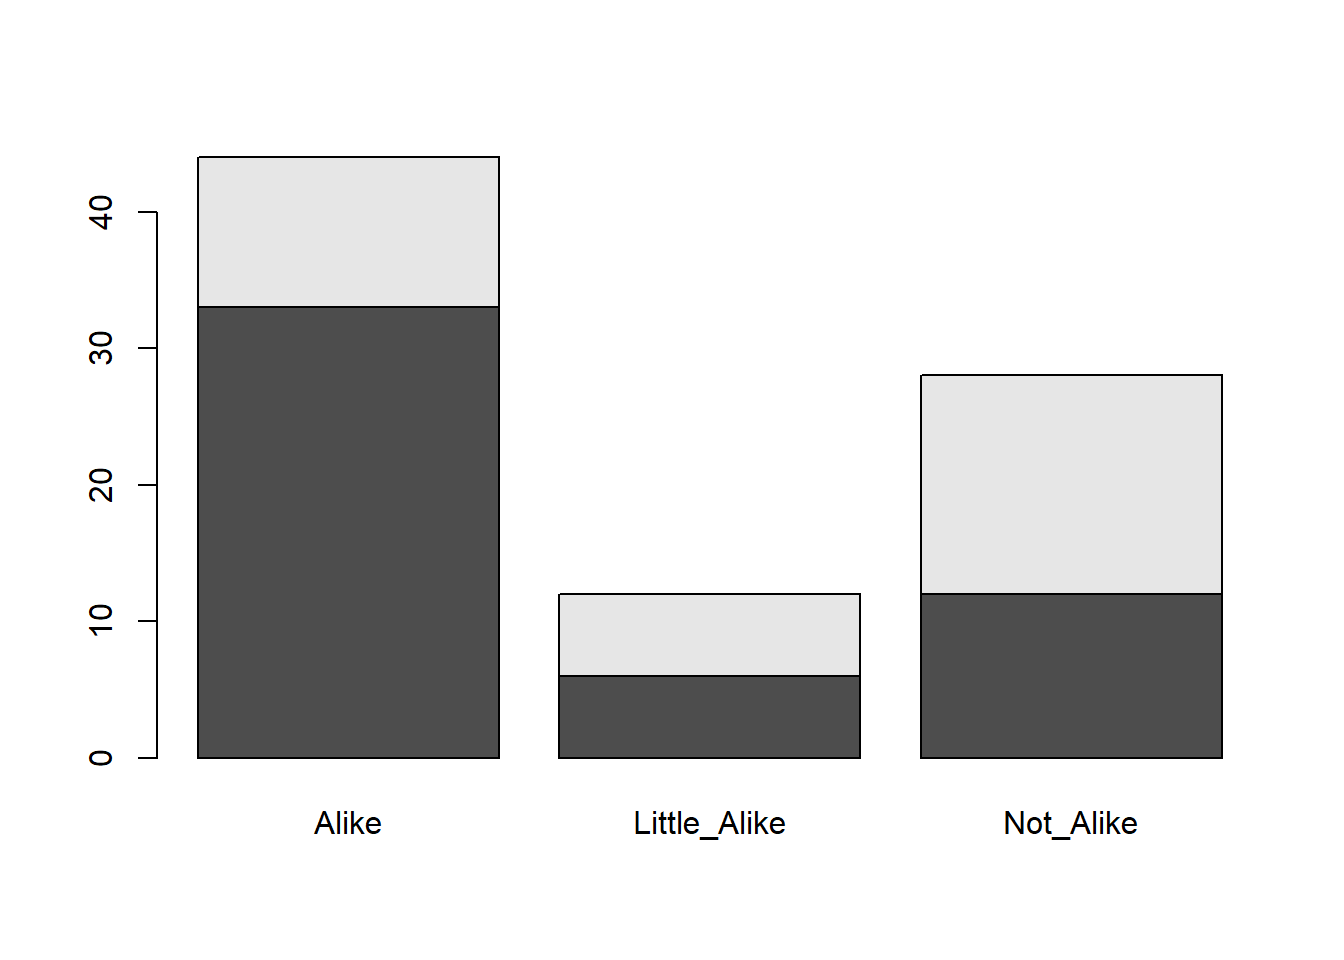
\includegraphics{VADeaths_files/figure-latex/unnamed-chunk-2-1.pdf}

\begin{Shaded}
\begin{Highlighting}[]
\FunctionTok{ggplot}\NormalTok{(}\AttributeTok{data =}\NormalTok{ VADeaths\_df,}
              \AttributeTok{mapping =} \FunctionTok{aes}\NormalTok{(}\AttributeTok{x =} \FunctionTok{interaction}\NormalTok{(Place, Gender), }
                            \AttributeTok{y =} \FunctionTok{rev}\NormalTok{(Rates), }
                            \AttributeTok{fill =}\NormalTok{ Age)) }\SpecialCharTok{+}
\FunctionTok{geom\_bar}\NormalTok{(}\AttributeTok{stat =} \StringTok{"identity"}\NormalTok{, }
         \AttributeTok{position =} \StringTok{"identity"}\NormalTok{)}
\end{Highlighting}
\end{Shaded}

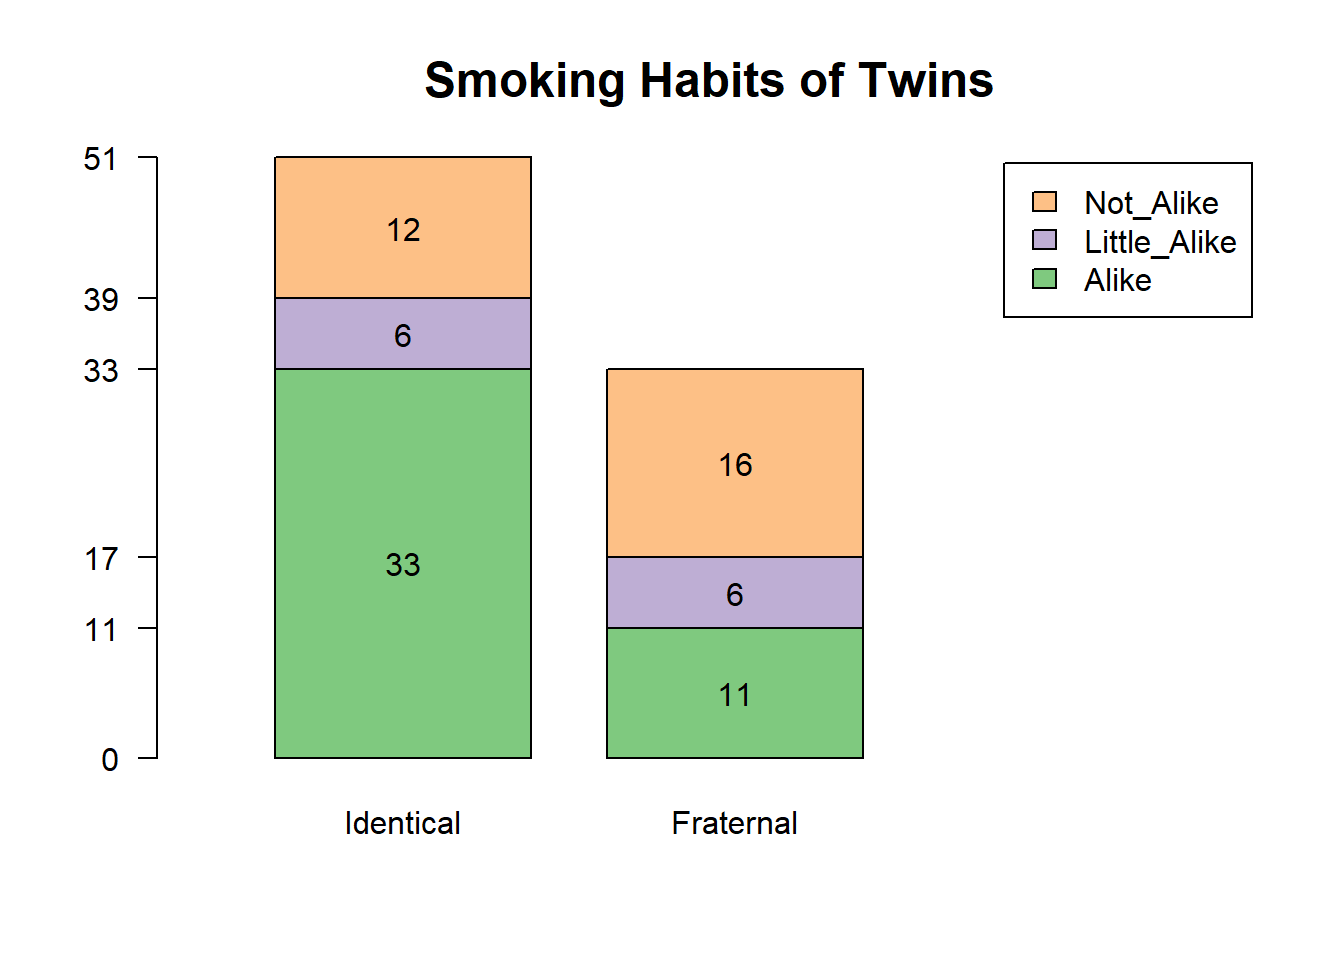
\includegraphics{VADeaths_files/figure-latex/unnamed-chunk-3-1.pdf}

\begin{Shaded}
\begin{Highlighting}[]
\FunctionTok{ggplot}\NormalTok{(}\AttributeTok{data =}\NormalTok{ VADeaths\_df,}
              \AttributeTok{mapping =} \FunctionTok{aes}\NormalTok{(}\AttributeTok{x =} \FunctionTok{interaction}\NormalTok{(Place, Gender), }
                            \AttributeTok{y =} \FunctionTok{rev}\NormalTok{(Rates), }
                            \AttributeTok{fill =}\NormalTok{ Age)) }\SpecialCharTok{+}
\FunctionTok{geom\_bar}\NormalTok{(}\AttributeTok{stat =} \StringTok{"identity"}\NormalTok{, }
         \AttributeTok{position =} \FunctionTok{position\_stack}\NormalTok{())}
\end{Highlighting}
\end{Shaded}

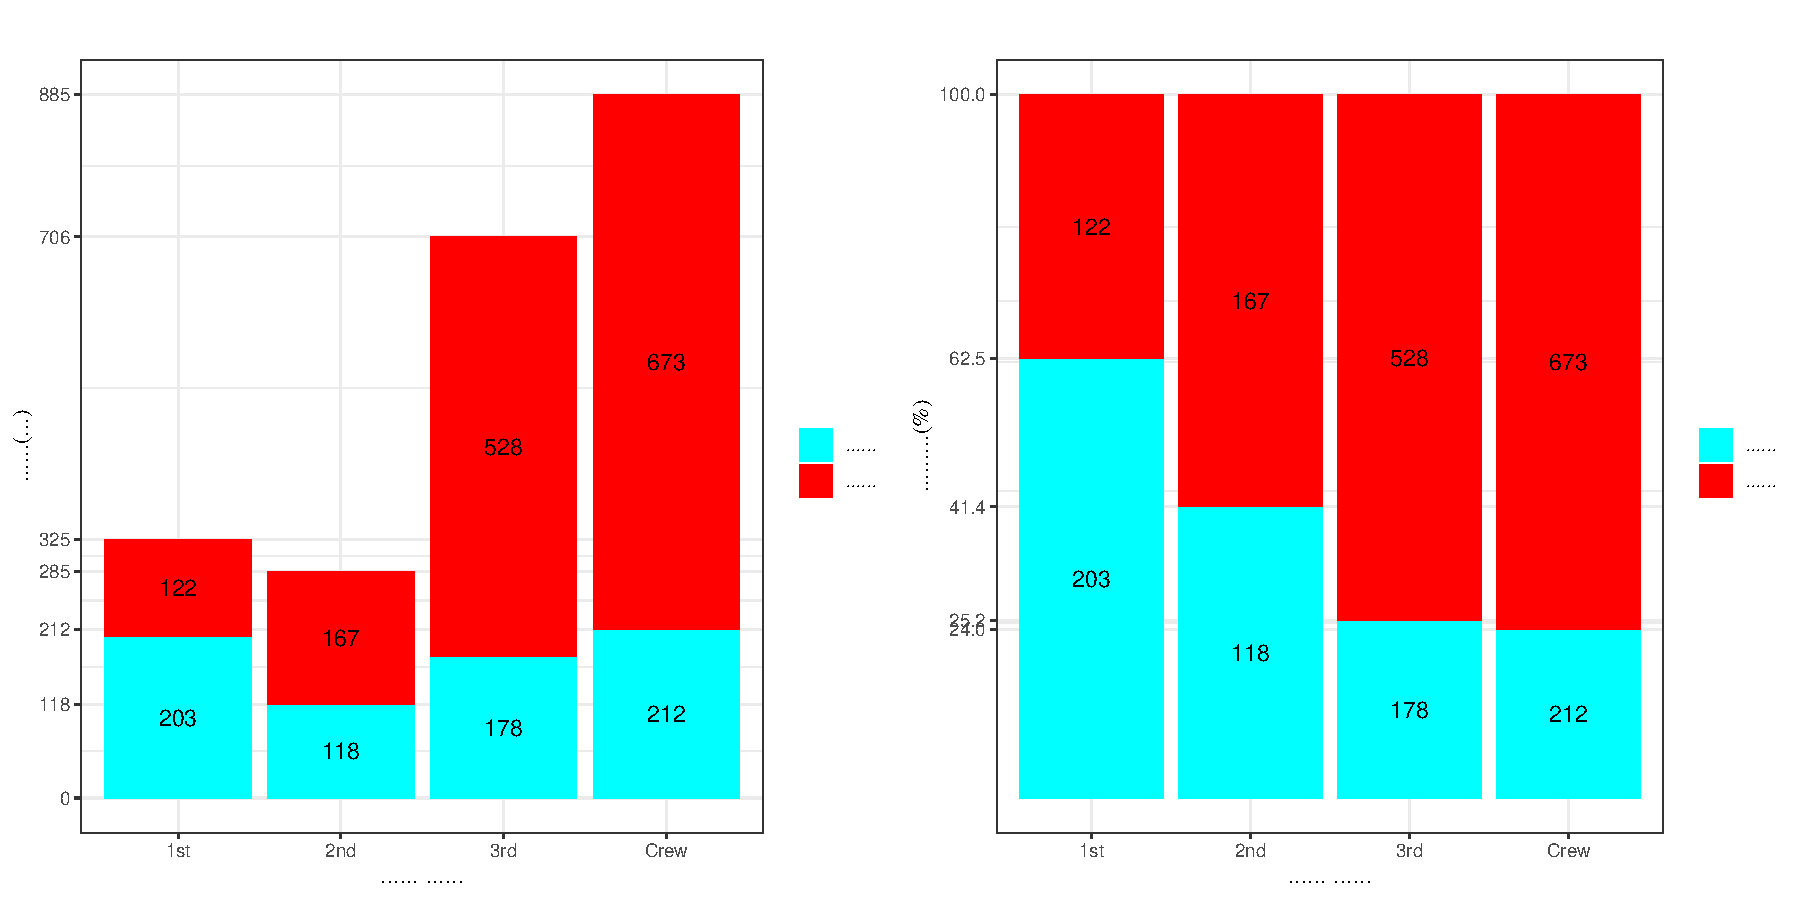
\includegraphics{VADeaths_files/figure-latex/unnamed-chunk-4-1.pdf}

\hypertarget{comments}{%
\subsection{Comments}\label{comments}}

학습한 내용에 대하여 가급적 상세하게 기술합니다.

\end{document}
